\documentclass[12pt]{report}
\usepackage[utf8]{inputenc}
\usepackage{amsmath}
\usepackage{amsfonts}
\usepackage{amssymb}
\usepackage[pdftex]{graphicx}
\usepackage{polski}

\usepackage{placeins}
\usepackage{epstopdf}
\usepackage{mathtools}
\usepackage{amsthm}
\usepackage{float}
\usepackage{tabularx}
\usepackage{titlesec}

\titleformat{\chapter}
{\Large\bfseries} % format
{}                % label
{0pt}             % sep
{\huge}           % before-code


\usepackage[left=2.50cm, right=2.50cm, top=2.50cm, bottom=2.50cm]{geometry}

\newcolumntype{C}[1]{>{\hsize=#1\hsize\centering\arraybackslash}X}
\newcolumntype{M}[1]{>{\centering\arraybackslash}m{#1}}

%opening
\title{\textbf{Laboratorium problemowe \\ Helikopter}}
\author{Maciej Cebula \\Marcin Kowalczyk \\ Daniel Rubak}
\date{}
\begin{document}
	
%	\fancypagestyle{plain}
%	{
%		% Usuń nagłówek i stopkę
%		\fancyhf{}
%		% Usuń linie.
%		\renewcommand{\headrulewidth}{0pt}
%		\renewcommand{\footrulewidth}{0pt}
%	}

	
	\setcounter{tocdepth}{2}
	
	\maketitle
	\tableofcontents
	\clearpage
		
		\renewcommand{\tablename}{Tabela}
		\renewcommand{\figurename}{Rys.}
		
	\chapter{Wstęp}

\section{Cel zajęć}

Celem zajęć było przygotowanie sterownika dla modelu helikoptera znajdującego się w laboratorium, którego uproszczony schemat przedstawiono na rysunku \ref{heli_model}. Jako środowisko programowe wykorzystano aplikację MATLAB wraz z pakietem Simulink. Wykorzystanie tych narzędzi polegało na komunikacji z rzeczywistym modelem helikoptera oraz wykonaniu modelu symulacyjnego.

\section{Obiekt sterowania}

Obiektem sterowania był model helikoptera o dwóch osiach swobody, który posiadał dwa wejścia (sterowanie silnikami, które napędzały śmigła) oraz dwa wyjścia (prędkość śmigła mierzona przez tachoprądnicę oraz położenie belki odczytywane z enkodera).


\begin{figure}[h!]
	\centering
	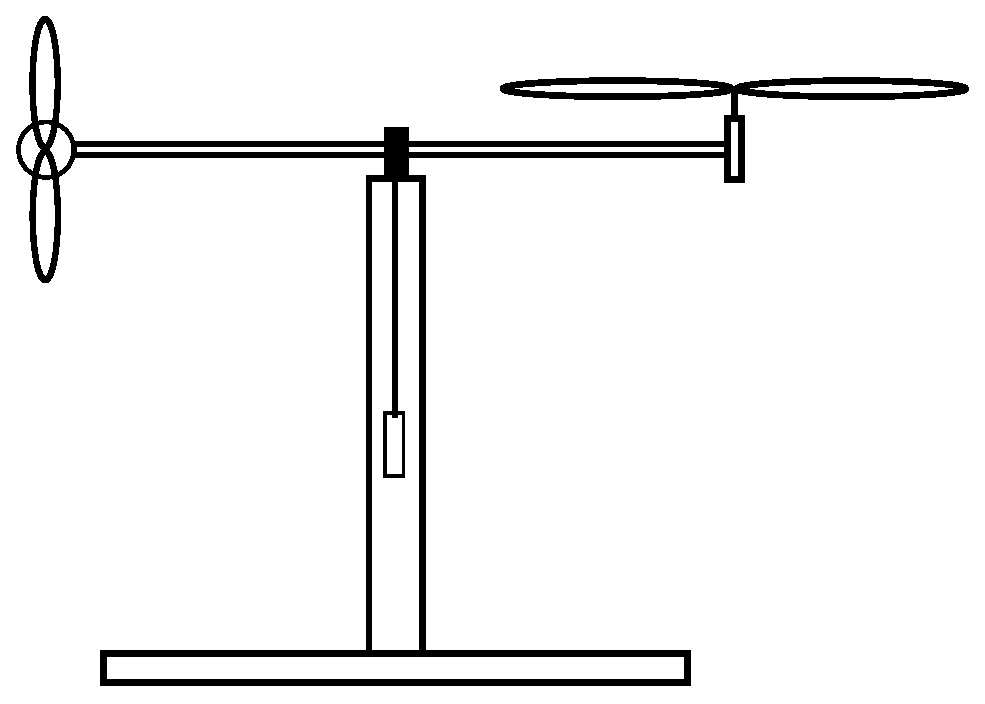
\includegraphics[scale = 0.6]{fig/model_helikoptera.eps}
	\caption		
	{Helikopter - schemat obiektu sterowania}
	\label{heli_model}
\end{figure} 

Na laboratorium zaimplementowano sterownik którego zadaniem było takie manipulowanie prędkościami silników helikoptera, aby ustabilizować obiekt w wybranym punkcie pracy. 

\section{Środowisko programowe}

Do implementacji sterownika wykorzystano środowisko programistyczne MATLAB/Simulink, w którego skład wchodziła biblioteka odpowiedzialna za komunikację z kartą RT-DAC4/PCI. Narzędzie to wykorzystano nie tylko do stworzenia panelu operacyjnego ale również do implementacji regulatorów, optymalizacji modelu i doboru odpowiednich nastaw. Panel operacyjny sterownika przedstawiono na rysunku \ref{heli_panel}.  

\begin{figure}[h!]
	\centering
	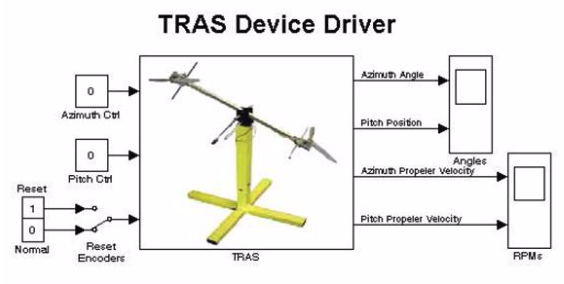
\includegraphics[scale = 1]{fig/heli_panel.png}
	\caption		
	{Panel operacyjny sterownika}
	\label{heli_panel}
\end{figure}
	\chapter{Identyfikacja}


\section{Identyfikacja parametrów śmigieł.}

W celu wyznaczenia dynamiki śmigieł helikoptera odpowiedzialnych za ruch odpowiednio względem osi pionowej - Pitch jak i poziomej - Azimuth, przeanalizowano odpowiedzi obiektu na wymuszenie w postaci skoku jednostkowego. Zmiana prędkości obrotowej każdego ze śmigieł, w reakcji na skokową zmianę napięcia zasilania, posłużyła do wyznaczenia parametrów transmitancji. Na bazie przeprowadzonych doświadczeń przyjęto, że każde ze śmigieł jest obiektem inercyjnym pierwszego rzędu w sytuacji gdy sygnałem wejściowym jest napięcie zasilania, a wyjściowym prędkość obrotowa. Do wyznaczenia parametrów tak przyjętego modelu wykorzystano metodę najmniejszych kwadratów. 

\begin{figure}[h!]
	\centering
	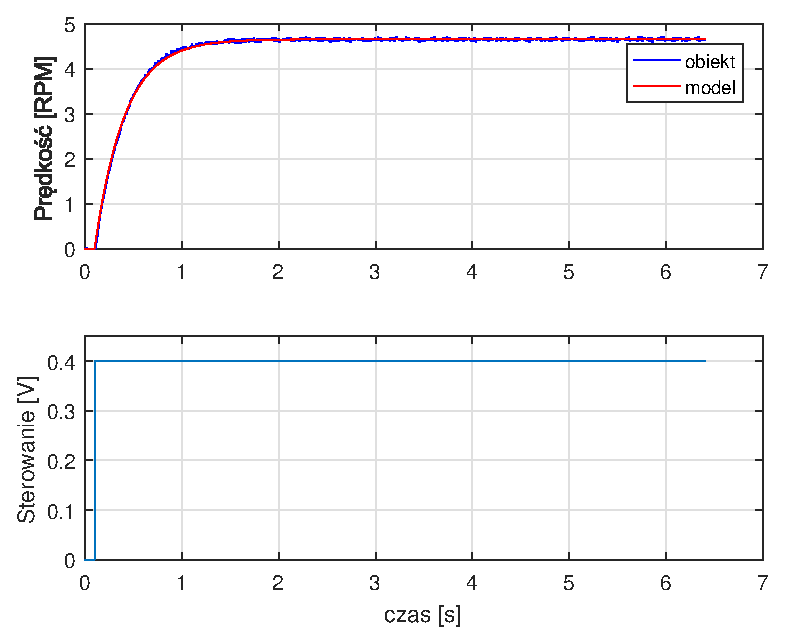
\includegraphics[scale = 1]{fig/Azimuth_iden.eps}
	\caption		
	{Charakterystyka śmigła oś pozioma.}
\end{figure} 
W przypadku osi poziomej model śmigła opisany jest następującą transmitancją:
\begin{equation}\label{key}
G(s) = \frac{K}{Ts + 1} = \frac{11.63}{0.31s + 1}
\end{equation}

\begin{figure}[h!]
	\centering
	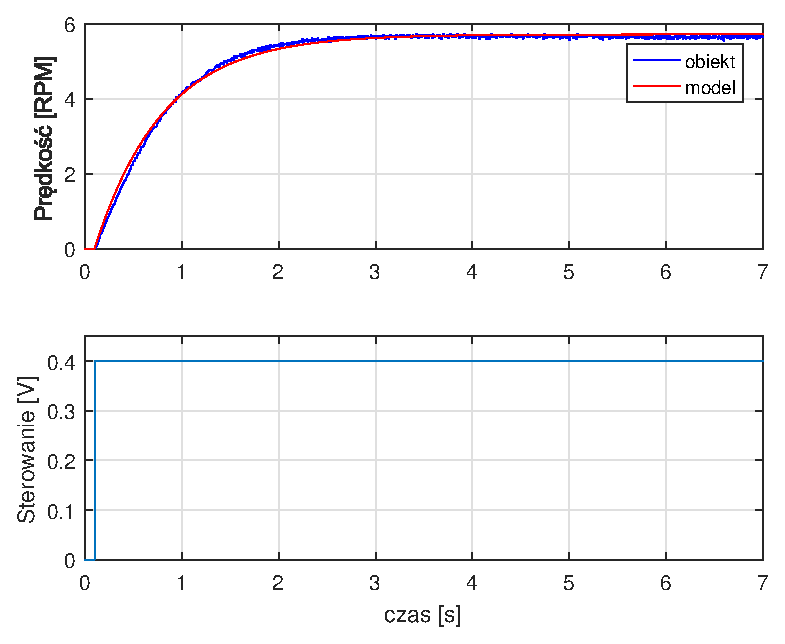
\includegraphics[scale = 1]{fig/Pitch_iden.eps}
	\caption		
	{Charakterystyka śmigła oś pionowa.}
\end{figure} 
Natomiast dla osi pionowej : 
\begin{equation}\label{key}
G(s) = \frac{K}{Ts + 1} = \frac{14.28}{0.71s + 1}
\end{equation}
 
 
\section{Charakterystyka statyczna helikoptera.}

Do wyznaczenia zależności generowanego momentu siły przez śmigło odpowiedzialne za ruch wzdłuż osi pionowej przeprowadzono eksperyment polegający na doczepianiu ciężarków o różnej masie z drugiej strony helikoptera i równoważeniu tak powstałego momentu siły przez odpowiednie dobranie prędkości obrotowej. W tabeli \ref{char_statyczna_tabela} podano otrzymane dane. 
\begin{table}[h]
	\caption{Porównanie poszczególnych regulatorów LQR.}
	\label{char_statyczna_tabela}
	\centering
	
	\begin{tabular}{|c|M{2.5cm}|M{2.5cm}|M{2.5cm}|}
		\hline
		Masa [g]&Prędkość [RPM]&Wsp. PWM [\%]&Moment siły [Nm]\\

		\hline
		0	&	7.1  & 63 & 0\\
		\hline
		15	&  6.3 &  51  & 0.0383\\
		\hline
		30	& 5.2	& 37 &  0.0765\\
		\hline
		45	& 3.75 & 32 &  0.1148\\
		\hline	
		60	& 0	&  0 &  0.1530\\
		\hline
		75	& -5.15	& -33  &   0.1913\\
		\hline
		90	&	-7.05 & -57 &   0.2296\\
		\hline
		105	&	-8.7 & -85 & 0.2678\\
		\hline
	\end{tabular}
\end{table}
Na podstawie zależności momentu siły od prędkości wyznaczono wielomian aproksymujący rzędu trzeciego opisanego zależnością : 
\begin{equation}\label{key}
M(v) = -0.0002v^3 -0.0009 v^2  - 0.0061v + 0.1571
\end{equation}

\begin{figure}[h!]
	\centering
	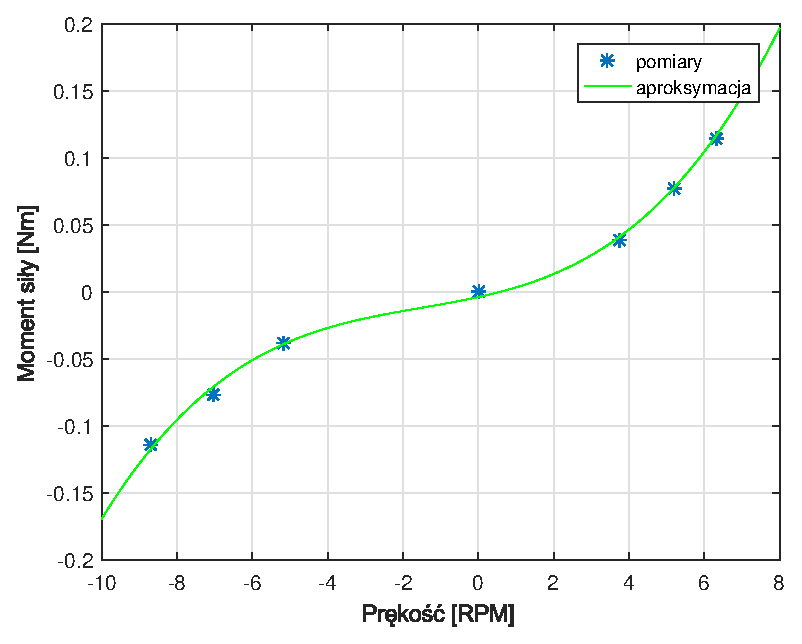
\includegraphics[scale = 1]{fig/char_statyczna.eps}
	\caption		
	{Charakterystyka statyczna śmigła oś pionowa.}
\end{figure} 

	
	\begin{thebibliography}{}
	
	%przykład 
	
%	\bibitem{pauluk 1}Pauluk, M.: 
%	\emph{Model matematyczny trójwymiarowej suwnicy.} W: \textbf{Automatyka} 2002 tom 6 s. 69-102, ISSN: 1429-3447
%	

	
\end{thebibliography}
	
\end{document}